\chapter{Introduction} \label{ch:1}
This chapter introduces ultra-intense lasers, gives applications of laser-accelerated protons, and presents an outline of the topics in this work.

\section{Lasers} \label{sec:lasers}

The word laser should actually be written as ``LASER'' because it is an acronym: light amplification by stimulated emission of radiation. Stimulated emission refers to Albert Einstein's 1917 paper which suggested photons (particles of light) could ``stimulate'' atoms to produce identical photons \cite{Einstein_1917_Quantum}. These identical photons would create a coherent light source which possess the same quantum-mechanical phase and wavelength. It was not until 1954 that Charles Townes and Arthur Schawlow first explored using stimulated emission to generate electromagnetic radiation\footnote{Electromagnetic radiation is just another word for light and is made up of oscillating electric and magnetic fields. The distance between adjacent wave crests in the fields is called the wavelength. Visible light has a wavelength between 400 and 700 nanometers and other forms of light (invisible to the naked eye) are similarly classified according to their wavelengths: radio, microwave, infra-red, ultra-violet, x-ray, gamma.} with a device called the \emph{maser} (because it produced \emph{microwave} wavelength light). In 1960, a similar device was constructed by Theodore Maiman at Hughes Research Laboratories that produced visible wavelength light \cite{Maiman_1960_Nature}. Maiman's device extended the maser to \emph{light} of different frequencies in what is now known as a \emph{laser}.

\begin{figure}
	\centering
	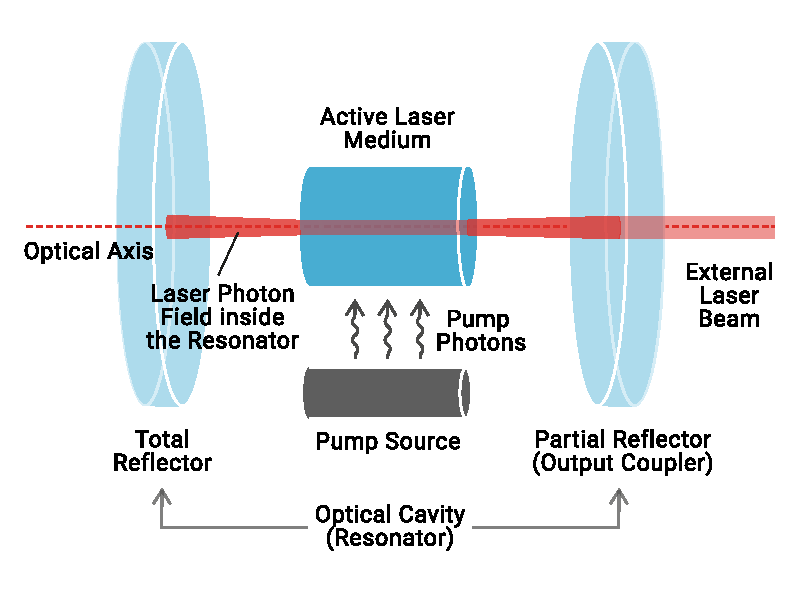
\includegraphics[width=0.75\linewidth]{planning/images/laser_gain.pdf}
	\caption{The components of a laser are depicted which include the pump source, active laser medium, and optical cavity. Image source: \cite{MeetOpticsPost}.}
	\label{fig:laser_gain}
\end{figure}

A typical laser operates by adding energy to some material, called the active lasing medium, from a pump source. The pump source can either be a strong flash of light or a pulse from a lower powered laser. The atoms in the medium absorb light which excites electrons to higher energy states. Over time, photons collide with excited atoms to stimulate emission of more photons. The medium is situated in an optical cavity (or resonator) composed of two reflecting mirrors that bounce these photons back and forth many times. With each reflection, photons pass back through the lasing medium, gaining more photon energy through stimulated emission as seen in \autoref{fig:laser_gain}. As a result, the active lasing medium is sometimes called the gain medium. Since one of the reflectors is only partially reflective, some of this laser light will pass through to become an external laser beam.

Lasers are best known for their ability to produce focused, high intensity light at a particular wavelength. Low powered lasers can be used as a laser pointer for a presentation, while higher powered lasers can cut solids. From both fundamental physics and industry perspectives, scientists are interested in increasing the intensity of lasers to explore various \gls{HEDS} phenomena. The most basic definition of intensity is

\begin{equation}
	\text{Intensity} = \frac{\text{Energy}}{\text{Area} \times \text{Time}}	
\end{equation}
So, for a given laser pulse, increasing the intensity could involve increasing the energy, decreasing the area (in terms of the surface that the laser beam hits), or decreasing the time. The energy can be increased by letting the laser stimulate emission of photons in the optical cavity with more passes. However, when the intensity in the cavity becomes too large, damage to the optical components (like the gain medium) can occur. In 1985, this problem was addressed by Donna Strickland and Gerard Mourou \cite{Strickland_1985_Optics} by first stretching an initial pulse in time before reaching the amplification stage in the gain medium. A stretched pulse can continue to gain energy while being sufficiently spread out (less intense) to not damage optical components as illustrated in 
\autoref{fig:cpa}. After amplification, the pulse is then compressed back into a shorter pulse. The clever use of gratings that separate light of different wavelengths allows pulses to easily be stretched and compressed in time. This method called \gls{CPA}, resulted in a nobel prize \cite{Nobel_2018}.

\begin{figure}
	\centering
	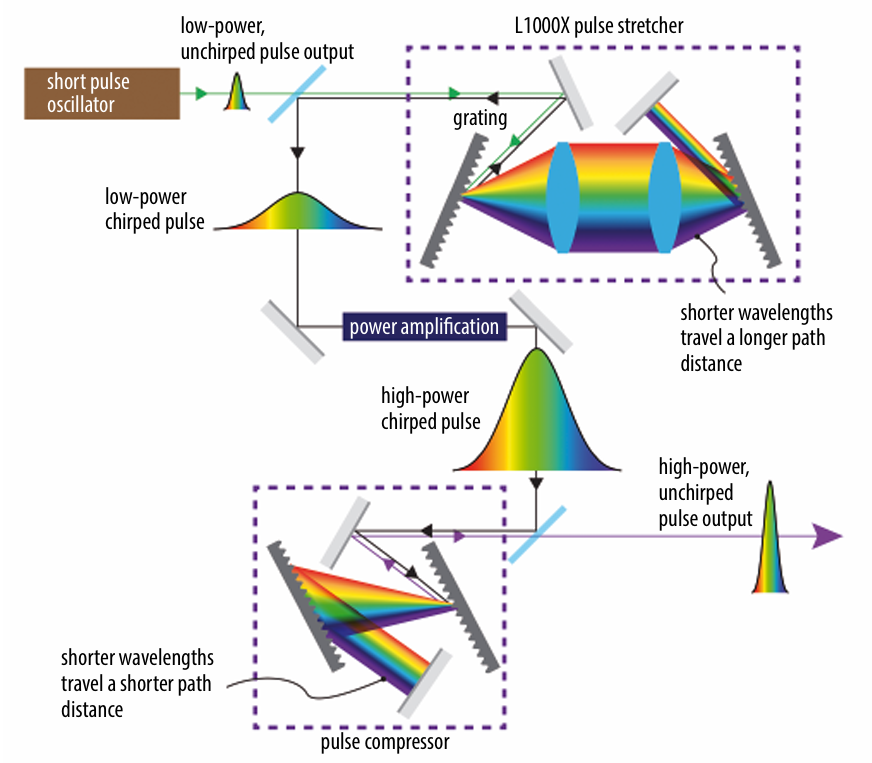
\includegraphics[width=0.9\linewidth]{planning/images/cpa.PNG}
	\caption{The stretch, amplification, and compression stages of chirped pulse amplification are depicted. Taken from \cite{Arrigoni_2019_Photonics}.}
	\label{fig:cpa}
\end{figure}
\gls{CPA} technology enabled lasers to produce high energy, extremely short femtosecond (a billionth of a millionth of a second) pulses that drove intensities into the relativistic regime where electrons can be accelerated to (nearly) the speed of light. The history of laser intensity since the production of the first laser in 1960 is depicted in \autoref{fig:laser_history}. The graph shows that between 1970-1985, laser intensities did not increase very much, but the invention of \gls{CPA} allowed intensities to increase 2-3 orders of magnitude every decade.

\begin{figure}
	\centering
	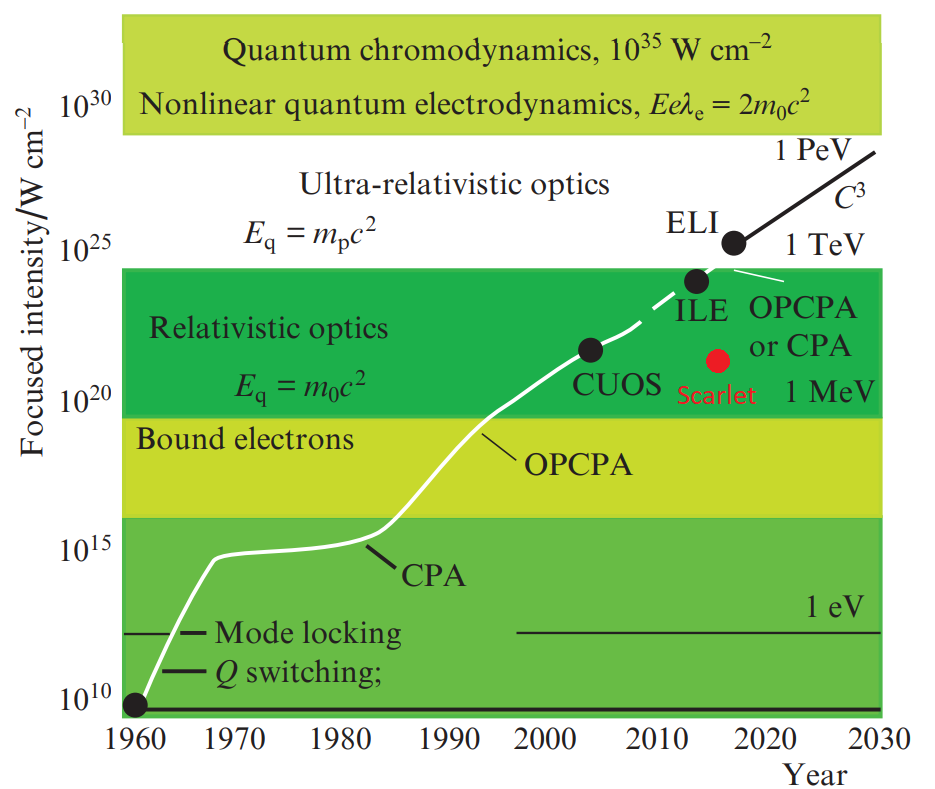
\includegraphics[width=0.75\linewidth]{planning/images/laser_history.PNG}
	\caption{History of focused laser intensities from the inception of the laser in 1960. The graph is labeled with intensity regimes, technological milestones, and acronyms of laser facilities. Modified from Figure 4 in Yakovlev \cite{Yakovlev_2014_QE} where OSU's Scarlet Laser was added.}
	\label{fig:laser_history}
\end{figure}

The laser at the Wright-Patterson Air Force base employs a titanium sapphire (Ti:Sapph) gain medium which is produced by doping (adding impurity) titanium ions in a sapphire\footnote{Corundrums are a mineral composed of aluminum oxide ($\text{Al}_2\text{O}_3$) with trace amounts of impurities that replace a small fraction of the aluminum ions. Blue sapphires have trace amounts of titanium and iron, while rubies have trace amounts of chromium.} crystal. These typically operate micron wavelength (infra-red) laser beams and are very commonly used in laser facilities across the globe. The Titan laser at \gls{JLF} uses a neodymium glass (Nd:glass) gain medium which is also configured for micron wavelengths. These two laser systems are the sites of the research discussed in this thesis.


\section{Applications}

The lasers described in the preceding section are used to study materials at high energy density scales. These laser-matter interactions are important for a variety of reasons. First, lasers can heat up materials to be as hot and dense as the core of the sun (if only for a tiny fraction of a second) which can provide astrophysical insights. Second, these hot, dense conditions are needed for nuclear fusion which is an extremely promising future source of clean energy (explored at places like the \gls{NIF}). Finally, laser-matter interactions can produce high energy, pulsed beams of protons, electrons, and ions. The most well-studied proton acceleration mechanism is called \gls{TNSA} whose physical origins will be explored more in \autoref{sec:acceleration}. 

During the course of my PhD, I have worked on ways to optimize the \gls{TNSA} mechanism for accelerating protons. This section highlights some of its most important applications: (1) proton therapy for cancer treatment, (2) proton radiography for imaging, and (3) ion beam analysis for materials characterization.


\subsection{Proton Therapy}

Cancer treatment is one of the largest medical challenges faced worldwide and cancer generally requires the use of harsh treatments like invasive surgery, chemotherapy, and immunotherapy. Another type of treatment is called radiotherapy and more than half of all people with cancer will receive it as a part of their medical care \cite{Mayo_2024_Cancer}. Typically, a large machine will provide a source of high energy x-rays that kills the tumor. However, this radiation does not discern whether the cells are cancerous or not -- healthy tissue along the radiation beam path surrounding the tumor will also be damaged. This damage can be mitigated by shooting many beams from different angles such that they overlap at the site of the tumor. In this way, the dose delivered in the beam overlap region will be significantly higher than the surrounding tissue. This approach is typically employed by situating the machine on a rotating ``gantry''.

As early as 1905, Bragg \cite{Bragg_1905_JOS} identified that charged particles have different properties than x-rays when passing through matter. Specifically, he identified that radium particles lost more energy (i.e. delivered a higher dose) at a lower speed. Physically, the slower the radium particles, the more time they have to scatter with individual atoms and the more energy they can deposit. This means that when radium first enters a material at its highest speed, it is losing energy slowly. In contrast, when radium is at a slow speed and about to stop, it is losing energy very quickly. In 1946, Wilson \cite{Wilson_1946_Rad} recognized that this property of charged particles could deliver a concentrated dose close to a tumor site. In \autoref{fig:bragg_curve}, these differences are explicitly highlighted between x-rays and proton beams traveling through water. It can be seen that the proton beam is sharply peaked at a distance of 24 centimeters, whereas the x-ray beam delivers a higher dose just a few centimeters in. One can see the advantage of protons quite readily from this picture -- if a tumor is located 24 centimeters into the body, the protons, comparatively to the x-rays, will deliver more energy at the tumor site and less energy to the surrounding tissue. Additionally, the dose delivered reduces to zero behind the tumor for protons which is not true for x-rays. The shape of the proton beam curve in this graph is appropriately referred to as a \emph{Bragg Curve} which peaks at the \emph{Bragg Peak}. 

The specifics of the depth-dose curve depend on the material that the particles are traveling through as well as initial energy of the protons (with higher energy protons traveling further into the material). These conditions are well-studied by empirical measurements of the \gls{SRIM} \cite{Ziegler_2010_SRIM} and can be combined with other techniques to achieve a depth-dose curve that not only peaks at different depths, but widens the region where the highest dose is delivered. The most modern form of proton therapy is called \gls{IMPT} whose intensities are modulated to optimally balance tumor dose and sparing of normal tissues \cite{Mohan_2022_PRO}. The first proton therapy center opened at the Loma Linda University Medical Center in California in 1990, but today there are more than 100 centers around the world (with more in the planning or construction stage) \cite{Mohan_2022_PRO}. 

\begin{figure}
	\centering
	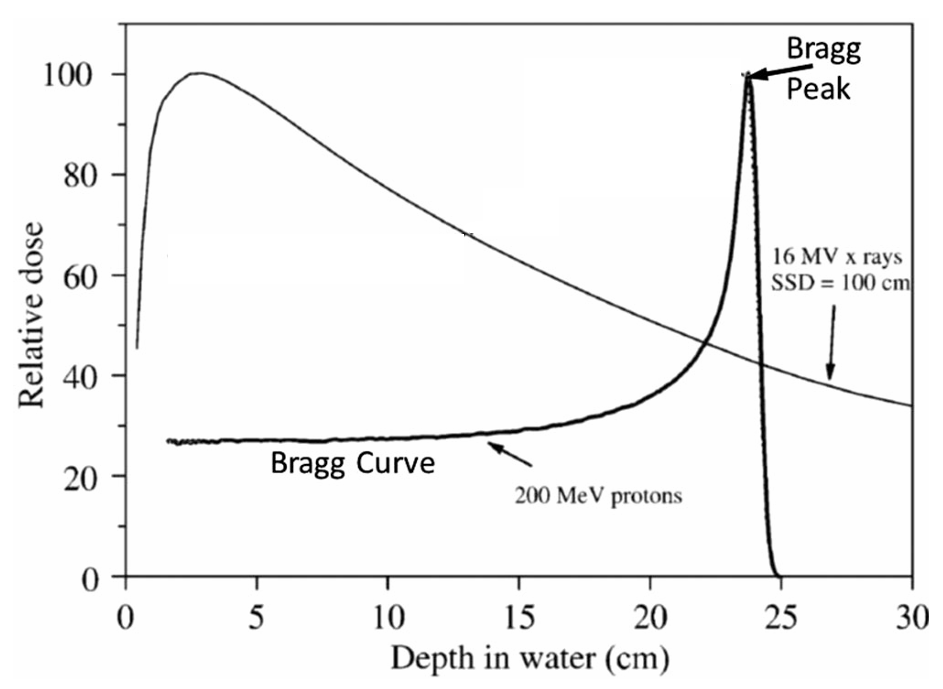
\includegraphics[width=0.75\linewidth]{planning/images/bragg_curve.PNG}
	\caption{The dose delivered as a function of depth traveled in water for two types of beams are depicted -- 200 MeV protons and 16 MV x-rays. Modified from Figure 1 in Mohan \cite{Mohan_2022_PRO}.}
	\label{fig:bragg_curve}
\end{figure}
 
Here in Columbus, \gls{OSUCCC}, in collaboration with Nationwide Children's Hospital, opened a 55,000 square foot proton therapy center in December of 2023 \cite{OSU_CCC} that uses \gls{IMPT}. Despite all the aformentioned benefits of proton therapy, the intial cost is tremendous -- \gls{OSUCCC} was a 100 million dollar investment. The significant cost demonstrates the value this could bring to Central Ohio. The facility is even outfitted with the capability to perform FLASH\footnote{Despite the capitalization, FLASH is not an acronym.} therapy which is a newer, experimental form of proton therapy. Compared to conventional methods, FLASH uses much higher dose-rates (i.e. greater than 40 Gy/s instead of less than 1 Gy/s) with much shorter exposure times (fractions of a second instead of minutes) for the same total dose. The higher dose-rate has been shown to reduce radiation-induced toxicity in healthy tissues in pre-clinical trials \cite{Matuszak_2022_Onc} and is currently under clinical trials \cite{OSU_CCC}. 

The conventional cyclotron accelerators used at \gls{OSUCCC} are extremely large and expensive which limits their availability to select locations globally. In recent years, it has been proposed that laser-based particle accelerators could be used to generate high energy protons. Laser-based sources can potentially produce even higher dose-rates ($\sim10^7$ Gy/s) and shorter exposure times (nanoseconds) for FLASH therapy \cite{Bin_2022_SciRep} to further reduce radiation-induced toxicity. Also, laser facilities could in principle be smaller and less costly. On the other hand, the technology is not matured enough to be considered in the near future \cite{Linz_2016_LaPB}. Current laser-based sources are typically only able to generate protons in the 10s of MeV reliably (as opposed to the 100s of MeV required for clinical operation) and exhibit poor repeatability of the laser pulse output. In addition, the conventional accelerators have already made significant strides in terms of reducing cost, increasing beam quality, and reducing size in recent years \cite{Linz_2016_LaPB} which is something laser-based sources will need to keep up with in the future. However, the potential of developing a smaller, lower cost, higher dose rate proton accelerator remains an important motivating factor for many laser-plasma physicists in the coming years.

\subsection{Laser Fusion and Proton Radiography}

Another use for protons is a diagnostic for laser fusion experiments. These use high powered lasers to compress a millimeter sized frozen pellet of hydrogen fuel\footnote{Specifically, heavier isotopes of hydrogen called deuterium and tritium are used} to such high temperatures and pressures similar to the core of the sun that the atomic nuclei fuse together into helium.

\begin{figure}
	\centering
	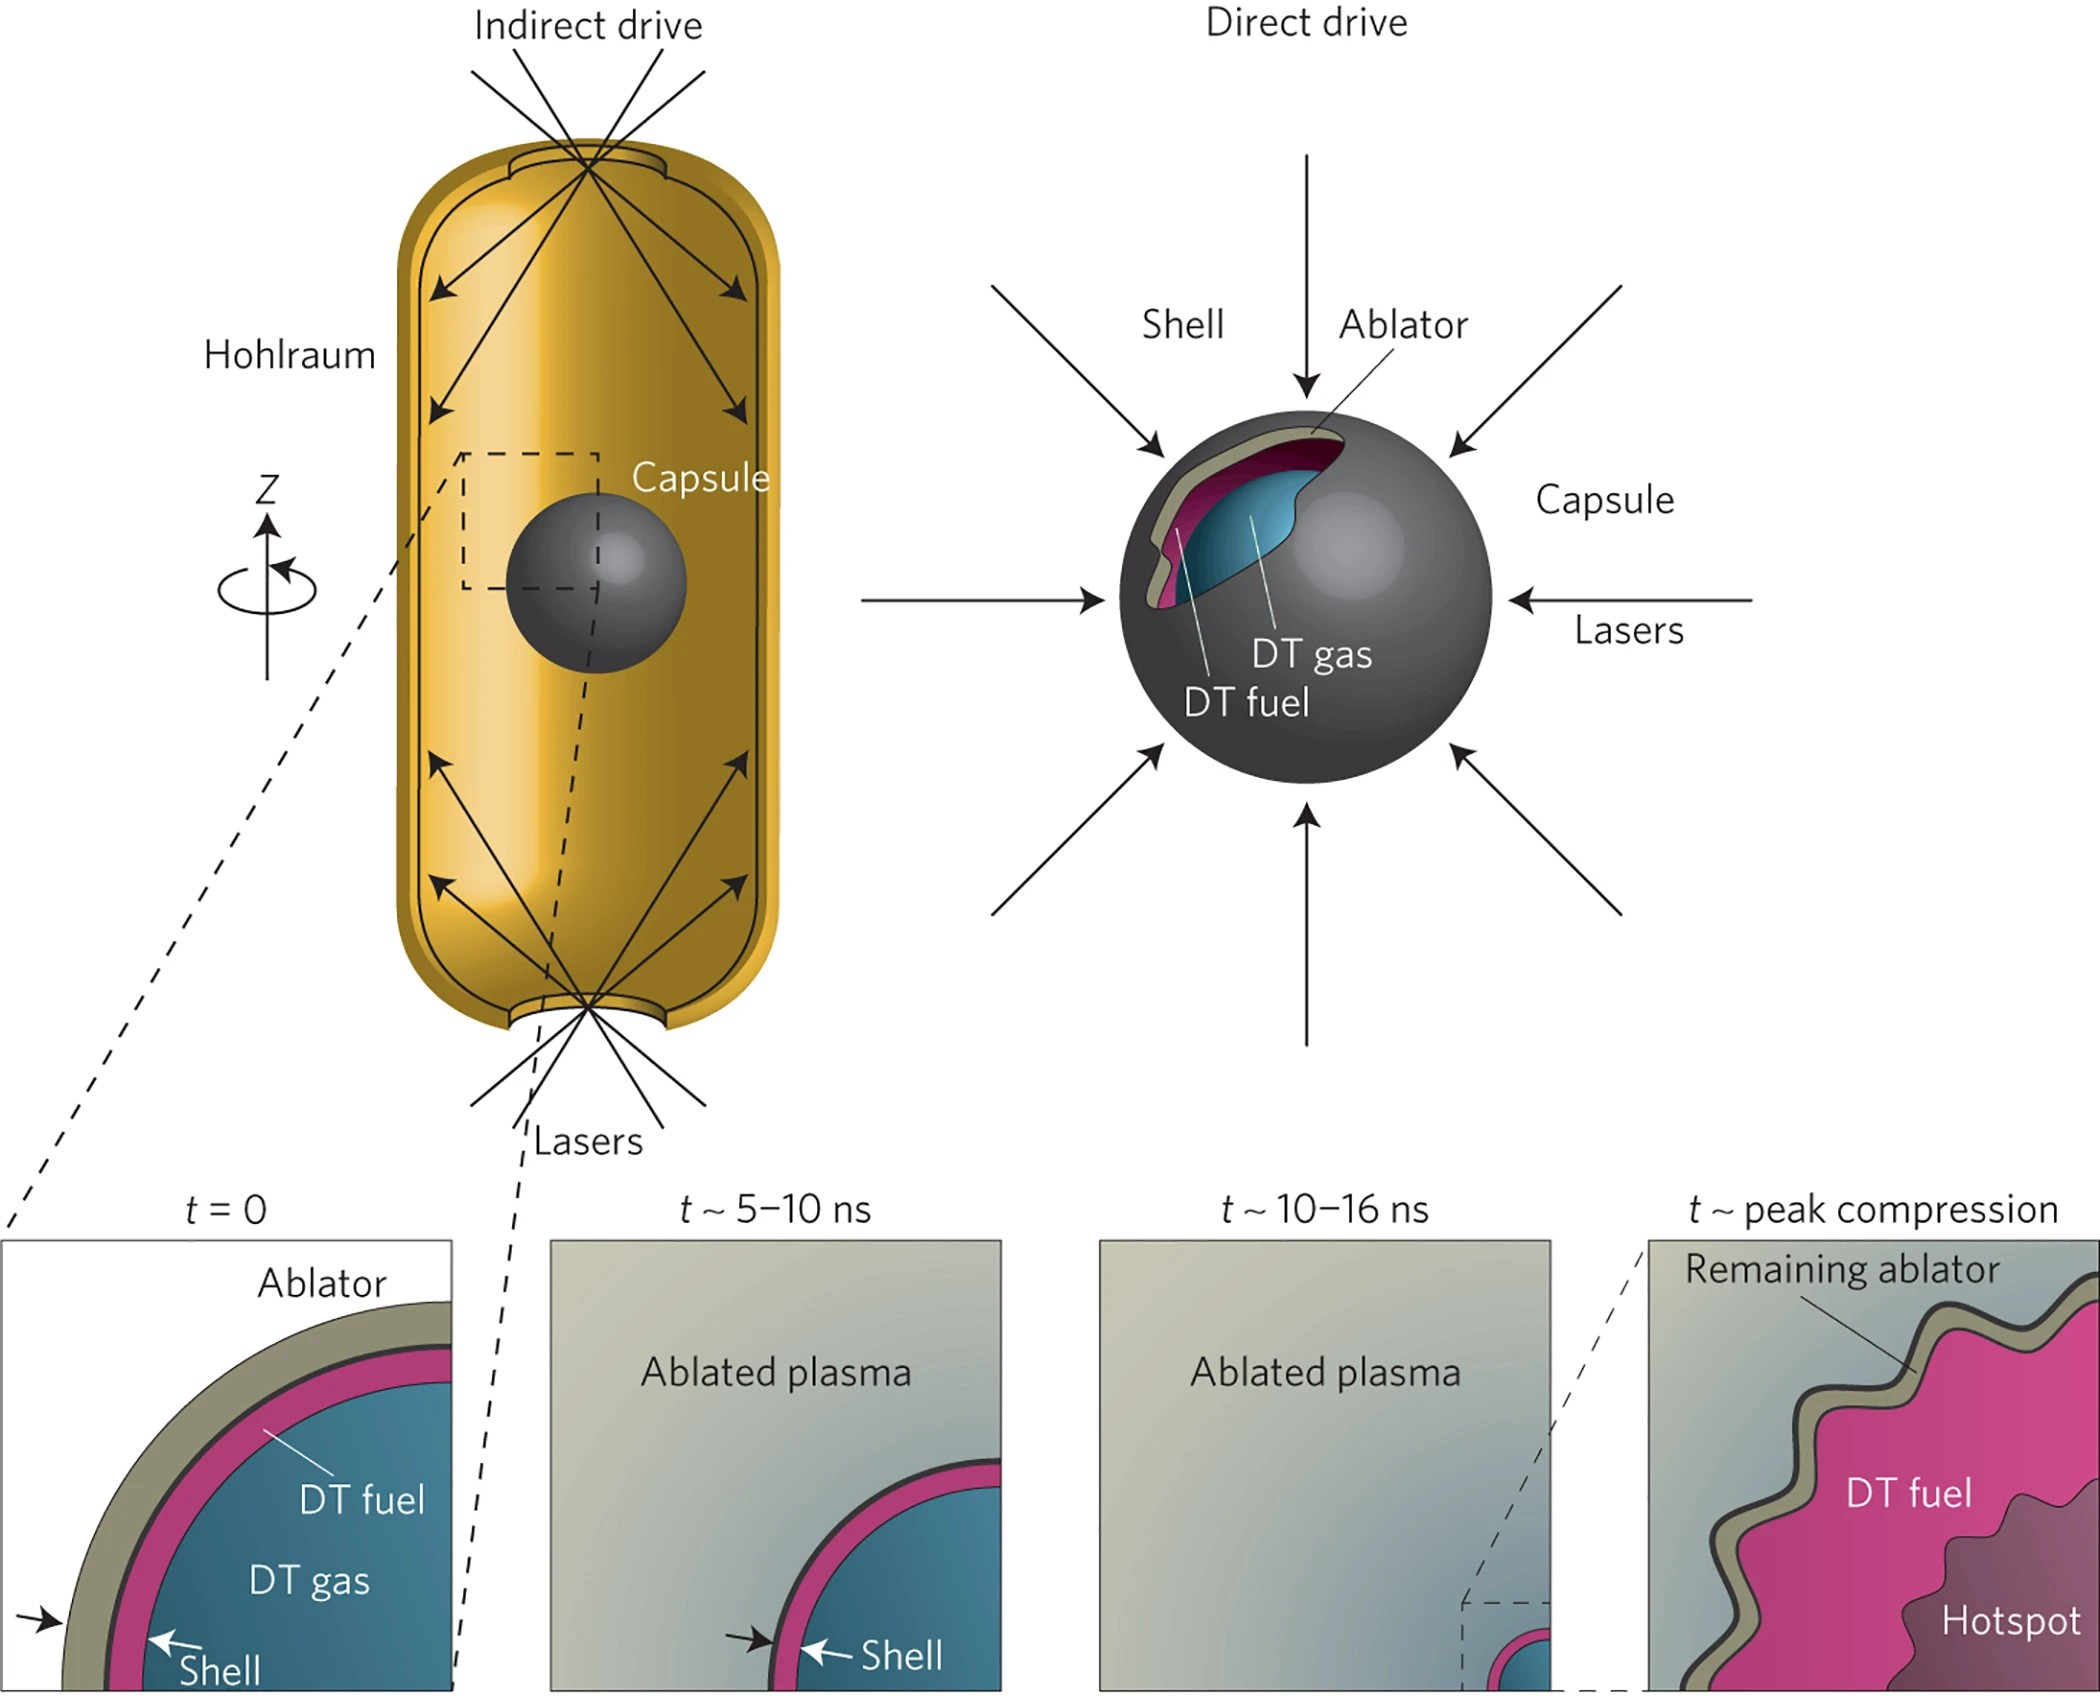
\includegraphics[width=0.9\linewidth]{planning/images/fusion.png}
	\caption{Visualization of two different approaches to laser fusion are depicted at the top. Lasers can irradiate the inside of a hollow gold can (called a hohlraum) to indirectly heat a fusion capsule or instead directly heat it. At the bottom, multiple stages of the fusion process are depicted including capsule ablation, compression, and burn. Taken from Figure 1 of Betti et al. \cite{Betti_2016_Nature}. }
	\label{fig:inertial_fusion}
\end{figure}

The fusion efforts are primarily conducted at two institutions in the United States. At the University of Rochester's \gls{LLE}, the OMEGA laser directly irradiates a fusion pellet in an approach called \emph{direct drive}. This is in contrast to the \gls{NIF} which indirectly compresses a fusion pellet by first irradiating a surrounding gold can in an approach called \emph{indirect drive}. These two approaches along with various fusion stages are illustrated in \autoref{fig:inertial_fusion}.

While visible light is typically used to image objects, other frequencies of light can be used as well. High frequency sources like x-rays are used at the dentist due to their ability to probe matter within your body. Radio waves reflect well off of electrically conductive materials like the metals in vehicles which make them ideal for military applications. Massive particles like protons can also be used and their different properties can be exploited to image things that cannot be done well with other types of radiation \cite{Schaeffer_2023_RevMod}. For example, the existence of the Bragg Peak in \autoref{fig:bragg_curve} enables proton images to have higher contrast than x-rays which deposit energy more uniformly.
 
For a laser fusion experiment with a nanosecond laser, an even shorter burst of protons would be needed to capture a ``still'' image or radiograph of the target at peak compression. Conventional sources of protons for radiography purposes are from linear accelerators like the pRad at \gls{LANL} that can accelerate up to 800 MeV protons \cite{LANL_PRAD} which can create microsecond or millisecond bursts of protons. In contrast, laser-driven proton sources can be generated in picosecond bursts through the \gls{TNSA} mechanism. Another advantage of these laser-accelerated proton beams is that they are emitted from a very small spot, on the order of microns, which is beneficial for obtaining a higher quality image \cite{Schaeffer_2023_RevMod}. This can be illustrated with a simple analogy to visible light -- the shadow produced from a small flashlight will have sharper edges than one produced from a larger fluorescent ceiling light.

With these considerations in mind, proton radiography has been demonstrated successfully at the \gls{NIF} through \gls{NIF-ARC} \cite{Simpson_2021_PPCF} and at OMEGA through \gls{OMEGA-EP} \cite{Zylstra_2012_RSI}. Both \gls{NIF-ARC} and \gls{OMEGA-EP} use a picosecond scale laser to produce \gls{TNSA} proton beams from laser-irradiated metallic foils and allow scientists to image fusion experiments on a timescale that would not be otherwise possible.

\subsection{Materials Characterization}

While protons can generate images through radiography, they can more generally tell us information about materials through a process called \gls{IBA}. \gls{IBA} allows scientists to probe material composition and surface structures with MeV ion beams which are appealing partly due to their non-destructive nature (comparatively to sources like x-rays) \cite{Passoni_2019_SciRep}. \gls{IBA} is currently implemented through old Van de Graaf and Tandem accelerator technology, but Passoni \cite{Passoni_2019_SciRep} argues that \gls{TNSA} proton beams can achieve the same result in a more compact, portable, and cheaper setup.

\begin{figure}
	\centering
	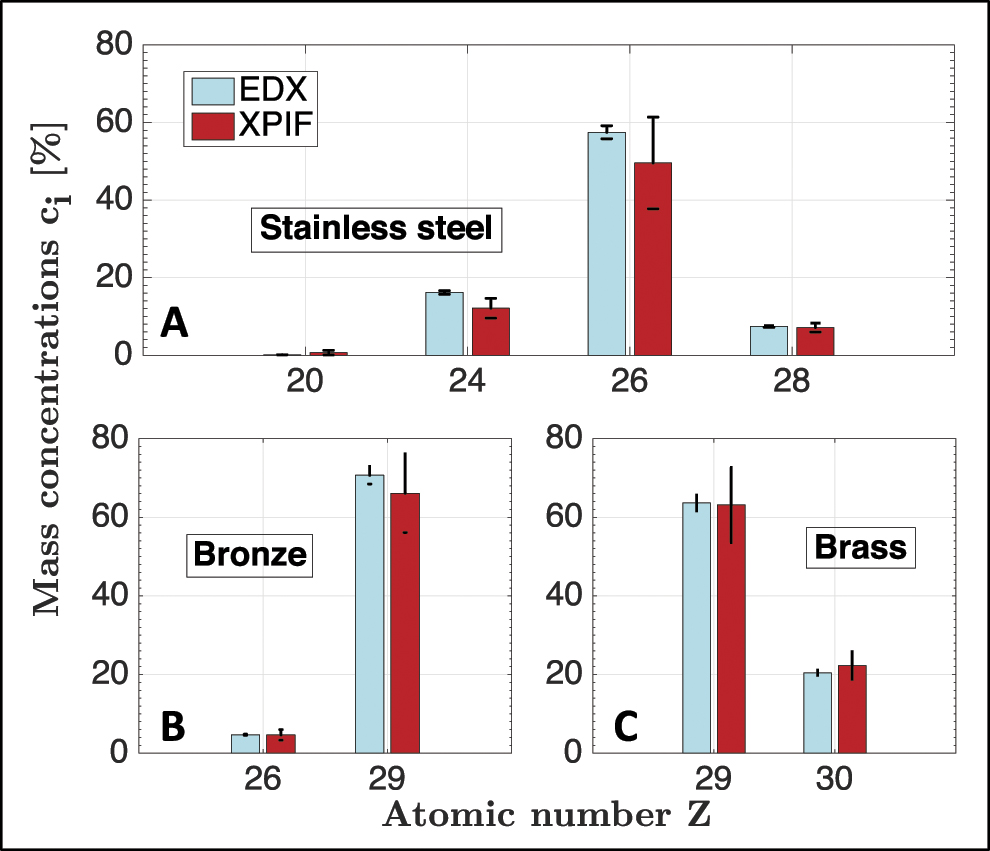
\includegraphics[width=0.6\linewidth]{planning/images/mass_concentration.jpg}
	\caption{Mass concentrations of three metal alloys are shown using two different techniques: Energy Dispersive x-ray Fluorescence (EDF) and X-ray and Particle-Induced Fluorescence. Taken from Figure 4 of Boivin et al. \cite{Boivin_2022_NJoP}.}
	\label{fig:mass_concentration}
\end{figure}

As a proof of principle, Boivin \cite{Boivin_2022_NJoP} used TNSA beams from the \gls{ALLS} laser facility in Canada to determine the elemental mass concentrations of three different metal alloys: stainless steel, bronze, and  brass using \gls{XPIF}. This is compared to a method called \gls{EDX} used in conjunction with a conventional mono-energetic electron beam and shown in \autoref{fig:mass_concentration}. Although XPIF has larger error bars than \gls{EDX}, both methods find good agreement with each other.

As a final point, \gls{TNSA} beams can be accompanied by other radiation sources like electrons, x-rays, and neutrons. Different materials characterization processes could, in principle, be used in conjunction with each other. While \gls{TNSA} beams are not the most common way to characterize materials today, they may emerge as an important tool for their ability to be pulsed at a high repetition rate and generated from a relatively compact system.

\section{Outline}
In the last decade, machine learning has emerged as an increasingly important tool\footnote{This is especially clear from the past few years of generative AI with tools like Chat-GPT.} for understanding the vast volume of data present in this world. Scientists have already been using machine learning in other fields to make new discoveries, but the field of laser-driven proton acceleration has only started to make use of it. This is because machine learning requires an immense amount of data to provide a true benefit \cite{Dopp_2023_HPLSE} and most modern laser systems only produce around one pulse per second (or less). Before my time, our group produced \gls{TNSA} proton beams in 2018 \cite{Morrison_2018_NJoP} from a laser system that sends 1000 pulses a second. With this many pulses, collecting large amounts of data now becomes a reality. However, to realize applications, the \gls{TNSA} proton beams need to be optimized for specific use cases. 

This work is a continuation of prior efforts in the group to computationally study \gls{TNSA} proton beams from Gregory Ngirmang, Joseph Smith, Nashad Rahman and others. In \autoref{ch:2} and \autoref{ch:3}, I give the physics and computational background needed to understand the main body of the dissertation. The bulk of my PhD work is summarized in \autoref{ch:5} which involved the construction of a synthetic proton acceleration dataset. This data was used as a testbed for assessing the feasibility of applying machine learning to possible future proton acceleration datasets. In \autoref{ch:4}, I detail the simulations I ran to corroborate the experimental findings of enhanced proton acceleration from the use of a split pulse. A future laser facility could possibility use the split pulse scheme as one of many optimizations to achieve a proton beam with desired properties. In \autoref{ch:6}, I detail my involvement in programming a machine learning feedback loop to automatically optimize accelerated electrons and protons from collected data. Finally, in \autoref{ch:7}, I conclude and give suggestions for future work.


